\documentclass[twoside]{book}

% Packages required by doxygen
\usepackage{calc}
\usepackage{doxygen}
\usepackage{graphicx}
\usepackage[utf8]{inputenc}
\usepackage{makeidx}
\usepackage{multicol}
\usepackage{multirow}
\usepackage{textcomp}
\usepackage[table]{xcolor}

% Font selection
\usepackage[T1]{fontenc}
\usepackage{mathptmx}
\usepackage[scaled=.90]{helvet}
\usepackage{courier}
\usepackage{amssymb}
\usepackage{sectsty}
\renewcommand{\familydefault}{\sfdefault}
\allsectionsfont{%
  \fontseries{bc}\selectfont%
  \color{darkgray}%
}
\renewcommand{\DoxyLabelFont}{%
  \fontseries{bc}\selectfont%
  \color{darkgray}%
}

% Page & text layout
\usepackage{geometry}
\geometry{%
  a4paper,%
  top=2.5cm,%
  bottom=2.5cm,%
  left=2.5cm,%
  right=2.5cm%
}
\tolerance=750
\hfuzz=15pt
\hbadness=750
\setlength{\emergencystretch}{15pt}
\setlength{\parindent}{0cm}
\setlength{\parskip}{0.2cm}
\makeatletter
\renewcommand{\paragraph}{%
  \@startsection{paragraph}{4}{0ex}{-1.0ex}{1.0ex}{%
    \normalfont\normalsize\bfseries\SS@parafont%
  }%
}
\renewcommand{\subparagraph}{%
  \@startsection{subparagraph}{5}{0ex}{-1.0ex}{1.0ex}{%
    \normalfont\normalsize\bfseries\SS@subparafont%
  }%
}
\makeatother

% Headers & footers
\usepackage{fancyhdr}
\pagestyle{fancyplain}
\fancyhead[LE]{\fancyplain{}{\bfseries\thepage}}
\fancyhead[CE]{\fancyplain{}{}}
\fancyhead[RE]{\fancyplain{}{\bfseries\leftmark}}
\fancyhead[LO]{\fancyplain{}{\bfseries\rightmark}}
\fancyhead[CO]{\fancyplain{}{}}
\fancyhead[RO]{\fancyplain{}{\bfseries\thepage}}
\fancyfoot[LE]{\fancyplain{}{}}
\fancyfoot[CE]{\fancyplain{}{}}
\fancyfoot[RE]{\fancyplain{}{\bfseries\scriptsize Generated on Wed Sep 14 2022 11\-:42\-:02 for V\-I\-S\-O\-R by Doxygen }}
\fancyfoot[LO]{\fancyplain{}{\bfseries\scriptsize Generated on Wed Sep 14 2022 11\-:42\-:02 for V\-I\-S\-O\-R by Doxygen }}
\fancyfoot[CO]{\fancyplain{}{}}
\fancyfoot[RO]{\fancyplain{}{}}
\renewcommand{\footrulewidth}{0.4pt}
\renewcommand{\chaptermark}[1]{%
  \markboth{#1}{}%
}
\renewcommand{\sectionmark}[1]{%
  \markright{\thesection\ #1}%
}

% Indices & bibliography
\usepackage{natbib}
\usepackage[titles]{tocloft}
\setcounter{tocdepth}{3}
\setcounter{secnumdepth}{5}
\makeindex

% Hyperlinks (required, but should be loaded last)
\usepackage{ifpdf}
\ifpdf
  \usepackage[pdftex,pagebackref=true]{hyperref}
\else
  \usepackage[ps2pdf,pagebackref=true]{hyperref}
\fi
\hypersetup{%
  colorlinks=true,%
  linkcolor=blue,%
  citecolor=blue,%
  unicode%
}

% Custom commands
\newcommand{\clearemptydoublepage}{%
  \newpage{\pagestyle{empty}\cleardoublepage}%
}


%===== C O N T E N T S =====

\begin{document}

% Titlepage & ToC
\hypersetup{pageanchor=false}
\pagenumbering{roman}
\begin{titlepage}
\vspace*{7cm}
\begin{center}%
{\Large V\-I\-S\-O\-R }\\
\vspace*{1cm}
{\large Generated by Doxygen 1.8.5}\\
\vspace*{0.5cm}
{\small Wed Sep 14 2022 11:42:02}\\
\end{center}
\end{titlepage}
\clearemptydoublepage
\tableofcontents
\clearemptydoublepage
\pagenumbering{arabic}
\hypersetup{pageanchor=true}

%--- Begin generated contents ---
\chapter{V\-I\-S\-O\-R}
\label{index}\hypertarget{index}{}The goal of this project is to direct near real-\/time satellite data regarding the optical properties of the surface ocean into operational ocean models and coupled ocean-\/atmosphere models. These satellite data are presently processed and distributed by the Naval Oceanographic Office (N\-A\-V\-O\-C\-E\-A\-N\-O) for warfighter support, however, at present there is no mechanism that would direct these data into the operational ocean models. The present suite of operational models uses either a static table of optical attenuation coefficients that is based on Jerlov’s early work (before the modern satellite era \mbox{[}Jerlov 1968\mbox{]}), or a static monthly climatology built from an obsolete N\-A\-S\-A mission (Sea\-Wi\-F\-S). As these operational models do not utilize any contemporaneous ocean optical attenuation data, the default attenuation and radiative transfer computations may result in gross errors for simulated upper ocean temperature structure, mixed layer depth, and substantial underestimates of air-\/sea thermal energy exchange rates. These errors will occur in spite of temperature data assimilation efforts because incorrect attenuation functions create structural problems in the way the ocean models calculate radiant heating throughout the upper water column. In coupled modeling systems, these errors will also impact the thermal energy balance within the simulated ocean-\/atmosphere systems and may have cascading effects on the forecasts for a wide range of tactically pertinent environmental variables, such as Electro-\/\-Magnetic (E\-M) duct heights. \hypertarget{index_my-intro}{}\section{V\-I\-S\-O\-R Overview}\label{index_my-intro}
\subsection*{Quick and Dirty}


\begin{DoxyItemize}
\item To build\-: ./scripts/build\-\_\-visor.sh
\item To run a test (must be customized, ./scripts/test\-\_\-netcdf.env)\-: ./scripts/test\-\_\-netcdfs.sh
\end{DoxyItemize}

\subsection*{Structure}


\begin{DoxyItemize}
\item ./\-Makefile -\/\-Linux P\-C's Makefile
\item ./\-Makefile\-\_\-\-D\-S\-R\-C -\/\-H\-P\-C Makefile
\item ./misc -\/directory containing material germane to software engineering of this project
\item ./jbooks -\/\-Jupyter lab files for basic debugging and origination of code.
\item ./screen\-\_\-visor.rc -\/\-Screen configuration to see execution of slicer.
\item ./scripts -\/directory with scripts used to\-:test, build, scan project.
\item ./build\-\_\-visor.sh -\/builds P\-C Makefile
\item ./build\-\_\-visor\-Cray.sh -\/builds D\-S\-R\-C Makefile, loads modules (Gordon, Conrad), for D\-S\-R\-C
\item ./build\-\_\-visor\-S\-G\-I.sh -\/builds D\-S\-R\-C Makefile, loads modules (Gaffney, Koehr), for D\-S\-R\-C
\item ./test$\ast$.sh -\/\-Various test routines
\item ./visor\-\_\-gops\-\_\-parser\-\_\-doxygen.dxy -\/\-Doxygen documentation generation configuration file
\item ./sonar-\/project.properties -\/\-Sonar\-Qube (D\-I2\-E, static code scanner) properties file.
\item ./sonar\-Scan\-\_\-visor.sh -\/\-Script to invoke sonar scan with key for this project.
\item ./profile.sh -\/\-Used to call various valgrind calls for code analysis
\item ./replicate\-Climo\-\_\-visor.ksh -\/\-Script for D\-S\-R\-C to replicate a single climatology to the entire year (12 months)
\item ./docs -\/\-S\-T\-I\-G, Design, A\-C\-G, and related documentation necessary for transition
\item ./src -\/actual source code
\begin{DoxyItemize}
\item ./visor\-\_\-gops\-\_\-climatology\-\_\-generator.c -\/\-Reads climatology and creates an N\-C\-O\-D\-A\-Q\-C compliant climo file(s)
\item ./visor\-\_\-gops\-\_\-parser.c -\/\-Reads Net\-C\-D\-F/\-H\-D\-F5 A\-P\-S generated satellite imagery and slices it for N\-C\-O\-D\-A\-Q\-C ingest
\item ./swapc\-\_\-bytes.c -\/\-Swaps bytes for N\-C\-O\-D\-A\-Q\-C D\-S\-R\-C Big-\/endian (required)
\item ./libll.c -\/\-Linked list tool used to store valid pixels in nodes on the heap.
\item ./lib\-Nav.c -\/\-Structure to store navigation data with basic support routines.
\item ./lib\-Product.c -\/\-Structure to store product data with basic support routines.
\item ./log.c -\/\-Logging framework from external source.
\end{DoxyItemize}
\item ./test -\/\-Directory containing results of testing and validation
\item ./\-Use\-Case -\/discrete information about data points to get against wrt the read
\item ./\-Test\-Case -\/actual execution results
\end{DoxyItemize}

\subsection*{Description}

Given a l3mapgen created file at 0.\-01 resolution produce a N\-C\-O\-D\-A-\/\-Q\-C compliant output file for ingest into the N\-C\-O\-D\-A system. Create a climatology file compliant with N\-C\-O\-D\-A-\/\-Q\-C expectations given a Net\-C\-D\-F based climatology file.

\subsection*{Libraries (Net\-C\-D\-F / H\-D\-F / H5)}

{\itshape Assumes access to A\-P\-S libraries in direct support of all Ocean Color efforts.}

A\-P\-S Libraries\-: {\ttfamily /net/americium/export/sw/linux-\/x86\-\_\-64-\/sl7/aps/local}

\subsection*{Reference}


\begin{DoxyItemize}
\item \href{https://confluence.di2e.net/display/NRL7331/VISOR}{\tt https\-://confluence.\-di2e.\-net/display/\-N\-R\-L7331/\-V\-I\-S\-O\-R}
\item \href{https://bitbucket.di2e.net/projects/NRL7331/repos/visor_gops_parser}{\tt https\-://bitbucket.\-di2e.\-net/projects/\-N\-R\-L7331/repos/visor\-\_\-gops\-\_\-parser/browse}
\end{DoxyItemize}

\subsection*{Versioning}

See the Design Document for details.

\subsection*{Operational file locations and job execution}


\begin{DoxyItemize}
\item Crontabs
\begin{DoxyItemize}
\item iridium (batch system master node) runs a job to pull N\-A\-V\-O\-C\-E\-A\-N\-O G\-O\-P\-S data locally
\item 00 07 $\ast$ $\ast$ $\ast$ /home/cwood/\-Documents/visor\-\_\-gops\-\_\-scripts/src/visor\-\_\-cron.sh $>$ /projects/socom/visor\-\_\-gops/logs/visor\-\_\-cron.log 2$>$\&1
\item data are stored in {\ttfamily /projects/socom/visor\-\_\-gops/db}
\item logs are stored in {\ttfamily /projects/socom/visor\-\_\-gops/logs}
\end{DoxyItemize}
\end{DoxyItemize}

\subsection*{T\-E\-S\-T C\-A\-S\-E\-S}


\begin{DoxyItemize}
\item {\ttfamily /projects/socom/\-N\-C\-O\-D\-A\-\_\-\-T\-E\-S\-T\-C\-A\-S\-E/2021\-\_\-\-T\-E\-S\-T}
\item Previous tests evidenced by D\-T\-G.
\end{DoxyItemize}

\subsection*{Critical Project Data}


\begin{DoxyItemize}
\item Climatology created by our team located at {\ttfamily /projects/socom/visor\-\_\-climatology/output/v3}
\item Source to build climatolog in this repository.
\item Source of data used to build output {\ttfamily /projects/socom/source/\-N\-A\-V\-O\-C\-E\-A\-N\-O\-\_\-\-J\-J}
\item Location on D\-S\-R\-C (gaffney,koehr) is {\ttfamily /p/work1/cwood/\-N\-C\-O\-D\-A\-Q\-C\-\_\-\-O\-P\-T\-I\-C\-S\-\_\-\-C\-L\-I\-M}, note that based on D\-S\-R\-C file schedules this can \char`\"{}suddenly\char`\"{} disappear without by-\/hands refresh.
\end{DoxyItemize}

\subsection*{D\-S\-R\-C Efforts}

See visor\-\_\-gops\-\_\-scripts repository. 
\chapter{V\-I\-S\-O\-R G\-O\-P\-S Parser / N\-C\-O\-D\-A\-Q\-C Writer}
\label{md_README}
\hypertarget{md_README}{}
/$\ast$! 
\chapter{Data Structure Index}
\section{Data Structures}
Here are the data structures with brief descriptions\-:\begin{DoxyCompactList}
\item\contentsline{section}{\hyperlink{structNavigation__Node}{Navigation\-\_\-\-Node} \\*Navigation structure with start points, overall size, and current index values }{\pageref{structNavigation__Node}}{}
\item\contentsline{section}{\hyperlink{structNode}{Node} \\*\hyperlink{structNode}{Node} structure to store a single pixel value with geospatial coordinates }{\pageref{structNode}}{}
\item\contentsline{section}{\hyperlink{structProduct}{Product} }{\pageref{structProduct}}{}
\item\contentsline{section}{\hyperlink{structProduct__Node}{Product\-\_\-\-Node} }{\pageref{structProduct__Node}}{}
\end{DoxyCompactList}

\chapter{File Index}
\section{File List}
Here is a list of all documented files with brief descriptions\-:\begin{DoxyCompactList}
\item\contentsline{section}{src/\hyperlink{libll_8c}{libll.\-c} \\*Contains definitions for Nodes used in a Linked List }{\pageref{libll_8c}}{}
\item\contentsline{section}{src/\hyperlink{libll_8h}{libll.\-h} \\*Contains definitions for Nodes used in a Linked List }{\pageref{libll_8h}}{}
\item\contentsline{section}{src/{\bfseries lib\-Nav.\-c} }{\pageref{libNav_8c}}{}
\item\contentsline{section}{src/\hyperlink{libNav_8h}{lib\-Nav.\-h} \\*Contains definitions for Navigation necessary for tracking position while processing each \char`\"{}slice\char`\"{} of an image }{\pageref{libNav_8h}}{}
\item\contentsline{section}{src/{\bfseries lib\-Product.\-c} }{\pageref{libProduct_8c}}{}
\item\contentsline{section}{src/\hyperlink{libProduct_8h}{lib\-Product.\-h} \\*Contains definitions for a \hyperlink{structProduct}{Product} structure necessary to hold salient meta-\/data related to a scientific data point. Information is gathered from the Net\-C\-D\-F/\-H\-D\-F5 file for persistence thus ensuring is does have to continually be accessed for the same data }{\pageref{libProduct_8h}}{}
\item\contentsline{section}{src/{\bfseries log.\-c} }{\pageref{log_8c}}{}
\item\contentsline{section}{src/\hyperlink{log_8h}{log.\-h} \\*Contains definitions for Nodes used in a Linked List }{\pageref{log_8h}}{}
\item\contentsline{section}{src/{\bfseries safe\-\_\-memcpy.\-c} }{\pageref{safe__memcpy_8c}}{}
\item\contentsline{section}{src/\hyperlink{safe__memcpy_8h}{safe\-\_\-memcpy.\-h} \\*Contains definitions for safe memory copy of strings }{\pageref{safe__memcpy_8h}}{}
\item\contentsline{section}{src/{\bfseries swapc\-\_\-bytes.\-c} }{\pageref{swapc__bytes_8c}}{}
\item\contentsline{section}{src/\hyperlink{swapc__bytes_8h}{swapc\-\_\-bytes.\-h} \\*Routines for swapping bytes due to endianess requirements of project }{\pageref{swapc__bytes_8h}}{}
\item\contentsline{section}{src/{\bfseries visor\-\_\-gops\-\_\-parser.\-c} }{\pageref{visor__gops__parser_8c}}{}
\end{DoxyCompactList}

\chapter{Data Structure Documentation}
\hypertarget{structNavigation__Node}{\section{Navigation\-\_\-\-Node Struct Reference}
\label{structNavigation__Node}\index{Navigation\-\_\-\-Node@{Navigation\-\_\-\-Node}}
}


Navigation structure with start points, overall size, and current index values.  




{\ttfamily \#include $<$lib\-Nav.\-h$>$}

\subsection*{Data Fields}
\begin{DoxyCompactItemize}
\item 
\hypertarget{structNavigation__Node_a6520a131effe5308becfddb288b0d19e}{int {\bfseries lon\-\_\-cols}}\label{structNavigation__Node_a6520a131effe5308becfddb288b0d19e}

\item 
\hypertarget{structNavigation__Node_a88f0e1c482d126e8d97d1caf945dd420}{float {\bfseries lon\-\_\-dpp}}\label{structNavigation__Node_a88f0e1c482d126e8d97d1caf945dd420}

\item 
\hypertarget{structNavigation__Node_a2d94f896d3e72975cd72fa9d0ff0b4e8}{float {\bfseries lon\-\_\-start}}\label{structNavigation__Node_a2d94f896d3e72975cd72fa9d0ff0b4e8}

\item 
\hypertarget{structNavigation__Node_a51233de3e050b595de21b7e3056c33c3}{int {\bfseries lon\-\_\-tot\-\_\-deg}}\label{structNavigation__Node_a51233de3e050b595de21b7e3056c33c3}

\item 
\hypertarget{structNavigation__Node_a068078b9590129d45116039976de5e08}{float {\bfseries lon\-\_\-abs\-\_\-start}}\label{structNavigation__Node_a068078b9590129d45116039976de5e08}

\item 
\hypertarget{structNavigation__Node_a44e00ebc6507634648ead4a0970e1bb8}{float {\bfseries lon\-\_\-offset}}\label{structNavigation__Node_a44e00ebc6507634648ead4a0970e1bb8}

\item 
\hypertarget{structNavigation__Node_aac6596efbc5911c30e5cc325bfc4dfd3}{float {\bfseries lon\-\_\-current}}\label{structNavigation__Node_aac6596efbc5911c30e5cc325bfc4dfd3}

\item 
\hypertarget{structNavigation__Node_afd2b6a7057238435dd972f4dcc0e42f6}{int {\bfseries lat\-\_\-rows}}\label{structNavigation__Node_afd2b6a7057238435dd972f4dcc0e42f6}

\item 
\hypertarget{structNavigation__Node_afc9fc0556971b7115aaaa3835b547670}{float {\bfseries lat\-\_\-dpp}}\label{structNavigation__Node_afc9fc0556971b7115aaaa3835b547670}

\item 
\hypertarget{structNavigation__Node_a89adf89f950fd9d8ec13b9fb503408f6}{float {\bfseries lat\-\_\-start}}\label{structNavigation__Node_a89adf89f950fd9d8ec13b9fb503408f6}

\item 
\hypertarget{structNavigation__Node_aaead85a1f756579271ea39e1367d3513}{int {\bfseries lat\-\_\-tot\-\_\-deg}}\label{structNavigation__Node_aaead85a1f756579271ea39e1367d3513}

\item 
\hypertarget{structNavigation__Node_a9bed2cf9d980020d0547972e4ddc031e}{float {\bfseries lat\-\_\-offset}}\label{structNavigation__Node_a9bed2cf9d980020d0547972e4ddc031e}

\item 
\hypertarget{structNavigation__Node_a3b9750f20ce78f2fba38c9ab9db46578}{float {\bfseries lat\-\_\-current}}\label{structNavigation__Node_a3b9750f20ce78f2fba38c9ab9db46578}

\item 
\hypertarget{structNavigation__Node_a626e9c31f566c861f986c0abf72d85ec}{int {\bfseries split\-\_\-idx}}\label{structNavigation__Node_a626e9c31f566c861f986c0abf72d85ec}

\item 
\hypertarget{structNavigation__Node_a6d5493a35d938fe5101ce61239eca51b}{int {\bfseries split\-\_\-coef}}\label{structNavigation__Node_a6d5493a35d938fe5101ce61239eca51b}

\item 
\hypertarget{structNavigation__Node_ae7cc0c19eafda3f1489f18227aade558}{float {\bfseries nw\-\_\-lon}}\label{structNavigation__Node_ae7cc0c19eafda3f1489f18227aade558}

\item 
\hypertarget{structNavigation__Node_a6dc9282ca1ecb484f86504d6be057cb4}{float {\bfseries nw\-\_\-lat}}\label{structNavigation__Node_a6dc9282ca1ecb484f86504d6be057cb4}

\item 
\hypertarget{structNavigation__Node_a71247a8aae788b7ce8589a109cb488b2}{float {\bfseries se\-\_\-lon}}\label{structNavigation__Node_a71247a8aae788b7ce8589a109cb488b2}

\item 
\hypertarget{structNavigation__Node_a332ea30a979bdbf7d4675b209001622b}{float {\bfseries se\-\_\-lat}}\label{structNavigation__Node_a332ea30a979bdbf7d4675b209001622b}

\end{DoxyCompactItemize}


\subsection{Detailed Description}
Navigation structure with start points, overall size, and current index values. 

Definition at line 18 of file lib\-Nav.\-h.



The documentation for this struct was generated from the following file\-:\begin{DoxyCompactItemize}
\item 
src/\hyperlink{libNav_8h}{lib\-Nav.\-h}\end{DoxyCompactItemize}

\hypertarget{structNode}{\section{Node Struct Reference}
\label{structNode}\index{Node@{Node}}
}


\hyperlink{structNode}{Node} structure to store a single pixel value with geospatial coordinates.  




{\ttfamily \#include $<$libll.\-h$>$}



Collaboration diagram for Node\-:\nopagebreak
\begin{figure}[H]
\begin{center}
\leavevmode
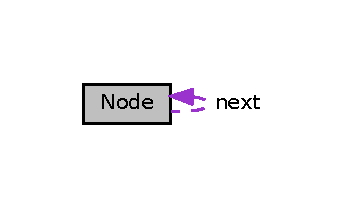
\includegraphics[width=165pt]{structNode__coll__graph}
\end{center}
\end{figure}
\subsection*{Data Fields}
\begin{DoxyCompactItemize}
\item 
\hypertarget{structNode_aef330e086c52cb0a14484b704a21f6c2}{float {\bfseries latitude}}\label{structNode_aef330e086c52cb0a14484b704a21f6c2}

\item 
\hypertarget{structNode_a6277484affb80e92218f52f5a38b8c09}{float {\bfseries longitude}}\label{structNode_a6277484affb80e92218f52f5a38b8c09}

\item 
\hypertarget{structNode_a4c704dbdd845bd145f41f9adaf485510}{float {\bfseries optics}}\label{structNode_a4c704dbdd845bd145f41f9adaf485510}

\item 
\hypertarget{structNode_a68d6e2a9d30f2f1280687f602411d545}{float {\bfseries optics\-\_\-log}}\label{structNode_a68d6e2a9d30f2f1280687f602411d545}

\item 
\hypertarget{structNode_af67b110ca1a258b793bf69d306929b22}{struct \hyperlink{structNode}{Node} $\ast$ {\bfseries next}}\label{structNode_af67b110ca1a258b793bf69d306929b22}

\end{DoxyCompactItemize}


\subsection{Detailed Description}
\hyperlink{structNode}{Node} structure to store a single pixel value with geospatial coordinates. 

Definition at line 18 of file libll.\-h.



The documentation for this struct was generated from the following file\-:\begin{DoxyCompactItemize}
\item 
src/\hyperlink{libll_8h}{libll.\-h}\end{DoxyCompactItemize}

\hypertarget{structProduct}{\section{Product Struct Reference}
\label{structProduct}\index{Product@{Product}}
}


\subsection{Detailed Description}
store information about the product such as offset, min/max value, etc. 

The documentation for this struct was generated from the following file\-:\begin{DoxyCompactItemize}
\item 
src/\hyperlink{libProduct_8h}{lib\-Product.\-h}\end{DoxyCompactItemize}

\hypertarget{structProduct__Node}{\section{Product\-\_\-\-Node Struct Reference}
\label{structProduct__Node}\index{Product\-\_\-\-Node@{Product\-\_\-\-Node}}
}
\subsection*{Data Fields}
\begin{DoxyCompactItemize}
\item 
\hypertarget{structProduct__Node_a5e2e88b162b3acc5745db0d534e9b762}{char $\ast$ {\bfseries product\-\_\-name}}\label{structProduct__Node_a5e2e88b162b3acc5745db0d534e9b762}

\item 
\hypertarget{structProduct__Node_ad3724e91d1b427b5e1859ca3947d0831}{float {\bfseries product\-\_\-scale\-\_\-factor}}\label{structProduct__Node_ad3724e91d1b427b5e1859ca3947d0831}

\item 
\hypertarget{structProduct__Node_a305c37e6c78a981f26c305f57975f4ab}{float {\bfseries product\-\_\-add\-\_\-offset}}\label{structProduct__Node_a305c37e6c78a981f26c305f57975f4ab}

\item 
\hypertarget{structProduct__Node_a5152eeed337daa783180765029f52fb9}{short {\bfseries product\-\_\-valid\-\_\-min}}\label{structProduct__Node_a5152eeed337daa783180765029f52fb9}

\item 
\hypertarget{structProduct__Node_ad60c20c6540b246d0ed992c1c7bc5c18}{short {\bfseries product\-\_\-valid\-\_\-max}}\label{structProduct__Node_ad60c20c6540b246d0ed992c1c7bc5c18}

\item 
\hypertarget{structProduct__Node_a8e4c5955bbd8cd6c6b2ce0cde9d6049f}{short {\bfseries product\-\_\-fill\-Value}}\label{structProduct__Node_a8e4c5955bbd8cd6c6b2ce0cde9d6049f}

\end{DoxyCompactItemize}


\subsection{Detailed Description}


Definition at line 48 of file lib\-Product.\-h.



The documentation for this struct was generated from the following file\-:\begin{DoxyCompactItemize}
\item 
src/\hyperlink{libProduct_8h}{lib\-Product.\-h}\end{DoxyCompactItemize}

\chapter{File Documentation}
\hypertarget{libll_8c}{\section{src/libll.c File Reference}
\label{libll_8c}\index{src/libll.\-c@{src/libll.\-c}}
}


Contains definitions for Nodes used in a Linked List.  


{\ttfamily \#include $<$stdio.\-h$>$}\\*
{\ttfamily \#include $<$stdlib.\-h$>$}\\*
{\ttfamily \#include $<$errno.\-h$>$}\\*
{\ttfamily \#include \char`\"{}log.\-h\char`\"{}}\\*
{\ttfamily \#include \char`\"{}libll.\-h\char`\"{}}\\*
Include dependency graph for libll.\-c\-:\nopagebreak
\begin{figure}[H]
\begin{center}
\leavevmode
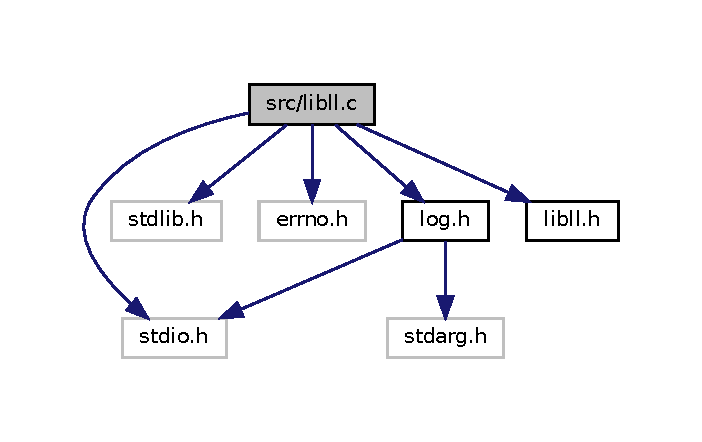
\includegraphics[width=337pt]{libll_8c__incl}
\end{center}
\end{figure}
\subsection*{Functions}
\begin{DoxyCompactItemize}
\item 
struct \hyperlink{structNode}{Node} $\ast$ \hyperlink{libll_8c_aa0fea1f9df88e0d0dd14ef3119aa437f}{New\-Node} ()
\begin{DoxyCompactList}\small\item\em Returns a pointer to memory specifically set up for node to represent the data. \end{DoxyCompactList}\item 
void \hyperlink{libll_8c_a783bf1a59e974223bd96eb069534d3ad}{Write\-List\-Items} (F\-I\-L\-E $\ast$$\ast$inc\-\_\-writefile, struct \hyperlink{structNode}{Node} $\ast$head)
\begin{DoxyCompactList}\small\item\em Given a node iterate through -\/$>$next and print\-: lat,lon,optics values to file. \end{DoxyCompactList}\item 
void \hyperlink{libll_8c_a66d59982b50fda3ea31a540f44731c6c}{Print\-List\-Items} (struct \hyperlink{structNode}{Node} $\ast$head)
\begin{DoxyCompactList}\small\item\em Given a node iterate through -\/$>$next and print\-: lat,lon,optics values to standard out. \end{DoxyCompactList}\item 
void \hyperlink{libll_8c_a91af3ff7b7b2fb602628b5741f440804}{Free\-List\-Items} (struct \hyperlink{structNode}{Node} $\ast$head)
\begin{DoxyCompactList}\small\item\em Given a node iterate through -\/$>$next free memory from each node. \end{DoxyCompactList}\item 
int \hyperlink{libll_8c_aa90ff9890b6196d9100e51d994c71640}{Count\-List\-Items} (struct \hyperlink{structNode}{Node} $\ast$input\-List)
\begin{DoxyCompactList}\small\item\em Given a node iterate through -\/$>$next counting until N\-U\-L\-L is reached and return the total. \end{DoxyCompactList}\end{DoxyCompactItemize}


\subsection{Detailed Description}
Contains definitions for Nodes used in a Linked List. V\-I\-S\-O\-R G\-O\-P\-S Parser Linked List Library \href{https://confluence.die2.net/display/NRL7331/VISOR}{\tt https\-://confluence.\-die2.\-net/display/\-N\-R\-L7331/\-V\-I\-S\-O\-R}

Copyright (c) 2020 Naval Research Lab (N\-R\-L)

This program is free software\-: you can redistribute it and/or modify it under the terms of the G\-N\-U General Public License as published by the Free Software Foundation, either version 3 of the License, or (at your option) any later version.

This program is distributed in the hope that it will be useful, but W\-I\-T\-H\-O\-U\-T A\-N\-Y W\-A\-R\-R\-A\-N\-T\-Y; without even the implied warranty of M\-E\-R\-C\-H\-A\-N\-T\-A\-B\-I\-L\-I\-T\-Y or F\-I\-T\-N\-E\-S\-S F\-O\-R A P\-A\-R\-T\-I\-C\-U\-L\-A\-R P\-U\-R\-P\-O\-S\-E. See the G\-N\-U General Public License for more details.

You should have received a copy of the G\-N\-U General Public License along with this program. If not, see \href{http://www.gnu.org/licenses/}{\tt http\-://www.\-gnu.\-org/licenses/}.

\begin{DoxyAuthor}{Author}
N\-R\-L, Code 7330 
\end{DoxyAuthor}
\begin{DoxyDate}{Date}
2019/05/31 Linked list library with basic support routines for reading 1 to N valid pixels in a satellite image and producing an N\-C\-O\-D\-A Q\-C compliant output.
\end{DoxyDate}
Added log scale capability to optics due to N\-C\-O\-D\-A downstream issues with the spectral shape of optics by transforming the data to a more bell shaped curve we avoid non-\/physical values (negatives) and keep optics more like S\-S\-T thus enabling more stock N\-C\-O\-D\-A$\ast$ utilization. Values will have to be reverted back once in the model prior to use. This ensures less code modification and keeps everything consistent within N\-C\-O\-D\-A$\ast$ proper.

\begin{DoxySeeAlso}{See Also}
\href{https://confluence.di2e.net/display/NRL7331/VISOR}{\tt https\-://confluence.\-di2e.\-net/display/\-N\-R\-L7331/\-V\-I\-S\-O\-R} 
\end{DoxySeeAlso}


Definition in file \hyperlink{libll_8c_source}{libll.\-c}.



\subsection{Function Documentation}
\hypertarget{libll_8c_aa90ff9890b6196d9100e51d994c71640}{\index{libll.\-c@{libll.\-c}!Count\-List\-Items@{Count\-List\-Items}}
\index{Count\-List\-Items@{Count\-List\-Items}!libll.c@{libll.\-c}}
\subsubsection[{Count\-List\-Items}]{\setlength{\rightskip}{0pt plus 5cm}int Count\-List\-Items (
\begin{DoxyParamCaption}
\item[{struct {\bf Node} $\ast$}]{input\-List}
\end{DoxyParamCaption}
)}}\label{libll_8c_aa90ff9890b6196d9100e51d994c71640}


Given a node iterate through -\/$>$next counting until N\-U\-L\-L is reached and return the total. 

Returns a count of nodes based on the node \char`\"{}head\char`\"{} passed in.


\begin{DoxyParams}{Parameters}
{\em \hyperlink{structNode}{Node}} & -\/ start node to free memory from \\
\hline
\end{DoxyParams}
\begin{DoxyReturn}{Returns}
int 
\end{DoxyReturn}


Definition at line 135 of file libll.\-c.

\hypertarget{libll_8c_a91af3ff7b7b2fb602628b5741f440804}{\index{libll.\-c@{libll.\-c}!Free\-List\-Items@{Free\-List\-Items}}
\index{Free\-List\-Items@{Free\-List\-Items}!libll.c@{libll.\-c}}
\subsubsection[{Free\-List\-Items}]{\setlength{\rightskip}{0pt plus 5cm}void Free\-List\-Items (
\begin{DoxyParamCaption}
\item[{struct {\bf Node} $\ast$}]{head}
\end{DoxyParamCaption}
)}}\label{libll_8c_a91af3ff7b7b2fb602628b5741f440804}


Given a node iterate through -\/$>$next free memory from each node. 

Iterates through each node from the \char`\"{}head\char`\"{} and frees memory as it goes.


\begin{DoxyParams}{Parameters}
{\em \hyperlink{structNode}{Node}} & -\/ start node to free memory from \\
\hline
\end{DoxyParams}
\begin{DoxyReturn}{Returns}
void 
\end{DoxyReturn}


Definition at line 118 of file libll.\-c.

\hypertarget{libll_8c_aa0fea1f9df88e0d0dd14ef3119aa437f}{\index{libll.\-c@{libll.\-c}!New\-Node@{New\-Node}}
\index{New\-Node@{New\-Node}!libll.c@{libll.\-c}}
\subsubsection[{New\-Node}]{\setlength{\rightskip}{0pt plus 5cm}struct {\bf Node}$\ast$ New\-Node (
\begin{DoxyParamCaption}
{}
\end{DoxyParamCaption}
)}}\label{libll_8c_aa0fea1f9df88e0d0dd14ef3119aa437f}


Returns a pointer to memory specifically set up for node to represent the data. 

Returns a newly minted \hyperlink{structNode}{Node}.


\begin{DoxyParams}{Parameters}
{\em None} & \\
\hline
\end{DoxyParams}
\begin{DoxyReturn}{Returns}
\hyperlink{structNode}{Node} 
\end{DoxyReturn}


Definition at line 49 of file libll.\-c.

\hypertarget{libll_8c_a66d59982b50fda3ea31a540f44731c6c}{\index{libll.\-c@{libll.\-c}!Print\-List\-Items@{Print\-List\-Items}}
\index{Print\-List\-Items@{Print\-List\-Items}!libll.c@{libll.\-c}}
\subsubsection[{Print\-List\-Items}]{\setlength{\rightskip}{0pt plus 5cm}void Print\-List\-Items (
\begin{DoxyParamCaption}
\item[{struct {\bf Node} $\ast$}]{head}
\end{DoxyParamCaption}
)}}\label{libll_8c_a66d59982b50fda3ea31a540f44731c6c}


Given a node iterate through -\/$>$next and print\-: lat,lon,optics values to standard out. 

Returns a printed list of nodes to standard output.


\begin{DoxyParams}{Parameters}
{\em \hyperlink{structNode}{Node}} & -\/ start node to print from \\
\hline
\end{DoxyParams}
\begin{DoxyReturn}{Returns}
void 
\end{DoxyReturn}


Definition at line 101 of file libll.\-c.

\hypertarget{libll_8c_a783bf1a59e974223bd96eb069534d3ad}{\index{libll.\-c@{libll.\-c}!Write\-List\-Items@{Write\-List\-Items}}
\index{Write\-List\-Items@{Write\-List\-Items}!libll.c@{libll.\-c}}
\subsubsection[{Write\-List\-Items}]{\setlength{\rightskip}{0pt plus 5cm}void Write\-List\-Items (
\begin{DoxyParamCaption}
\item[{F\-I\-L\-E $\ast$$\ast$}]{inc\-\_\-writefile, }
\item[{struct {\bf Node} $\ast$}]{head}
\end{DoxyParamCaption}
)}}\label{libll_8c_a783bf1a59e974223bd96eb069534d3ad}


Given a node iterate through -\/$>$next and print\-: lat,lon,optics values to file. 

Outputs ndoe meta-\/data (lat,lon,optics) to the file provided for output.


\begin{DoxyParams}{Parameters}
{\em F\-I\-L\-E} & -\/ double pointer to output file \\
\hline
{\em \hyperlink{structNode}{Node}} & -\/ start node to print from \\
\hline
\end{DoxyParams}
\begin{DoxyReturn}{Returns}
void 
\end{DoxyReturn}


Definition at line 69 of file libll.\-c.


\hypertarget{libll_8h}{\section{src/libll.h File Reference}
\label{libll_8h}\index{src/libll.\-h@{src/libll.\-h}}
}


Contains definitions for Nodes used in a Linked List.  


This graph shows which files directly or indirectly include this file\-:\nopagebreak
\begin{figure}[H]
\begin{center}
\leavevmode
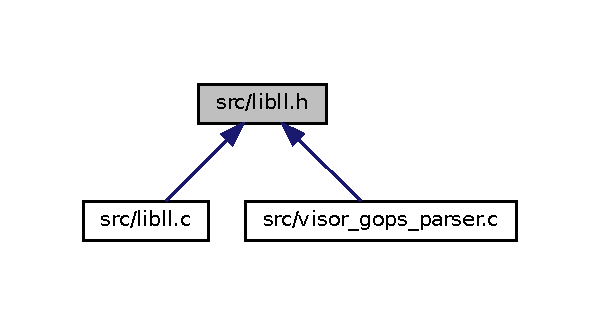
\includegraphics[width=288pt]{libll_8h__dep__incl}
\end{center}
\end{figure}
\subsection*{Data Structures}
\begin{DoxyCompactItemize}
\item 
struct \hyperlink{structNode}{Node}
\begin{DoxyCompactList}\small\item\em \hyperlink{structNode}{Node} structure to store a single pixel value with geospatial coordinates. \end{DoxyCompactList}\end{DoxyCompactItemize}
\subsection*{Functions}
\begin{DoxyCompactItemize}
\item 
struct \hyperlink{structNode}{Node} $\ast$ \hyperlink{libll_8h_aa0fea1f9df88e0d0dd14ef3119aa437f}{New\-Node} ()
\begin{DoxyCompactList}\small\item\em Returns a newly minted \hyperlink{structNode}{Node}. \end{DoxyCompactList}\item 
int \hyperlink{libll_8h_a14ccd3536ae7a080ee36948426fd7f70}{Count\-List\-Items} (struct \hyperlink{structNode}{Node} $\ast$head)
\begin{DoxyCompactList}\small\item\em Returns a count of nodes based on the node \char`\"{}head\char`\"{} passed in. \end{DoxyCompactList}\item 
void \hyperlink{libll_8h_a66d59982b50fda3ea31a540f44731c6c}{Print\-List\-Items} (struct \hyperlink{structNode}{Node} $\ast$head)
\begin{DoxyCompactList}\small\item\em Returns a printed list of nodes to standard output. \end{DoxyCompactList}\item 
void \hyperlink{libll_8h_a91af3ff7b7b2fb602628b5741f440804}{Free\-List\-Items} (struct \hyperlink{structNode}{Node} $\ast$head)
\begin{DoxyCompactList}\small\item\em Iterates through each node from the \char`\"{}head\char`\"{} and frees memory as it goes. \end{DoxyCompactList}\item 
void \hyperlink{libll_8h_a6803d4a058156a21a7beeebb86254ec3}{Write\-List\-Items} (F\-I\-L\-E $\ast$$\ast$inc\-\_\-outputfile, struct \hyperlink{structNode}{Node} $\ast$head)
\begin{DoxyCompactList}\small\item\em Outputs ndoe meta-\/data (lat,lon,optics) to the file provided for output. \end{DoxyCompactList}\end{DoxyCompactItemize}


\subsection{Detailed Description}
Contains definitions for Nodes used in a Linked List. \begin{DoxyAuthor}{Author}
N\-R\-L, Code 7330 
\end{DoxyAuthor}
\begin{DoxyDate}{Date}
2019/05/31 Linked list library with basic support routines for reading 1 to N valid pixels in a satellite image and producing an N\-C\-O\-D\-A Q\-C compliant output.
\end{DoxyDate}
\begin{DoxySeeAlso}{See Also}
\href{https://confluence.di2e.net/display/NRL7331/VISOR}{\tt https\-://confluence.\-di2e.\-net/display/\-N\-R\-L7331/\-V\-I\-S\-O\-R} 
\end{DoxySeeAlso}


Definition in file \hyperlink{libll_8h_source}{libll.\-h}.



\subsection{Function Documentation}
\hypertarget{libll_8h_a14ccd3536ae7a080ee36948426fd7f70}{\index{libll.\-h@{libll.\-h}!Count\-List\-Items@{Count\-List\-Items}}
\index{Count\-List\-Items@{Count\-List\-Items}!libll.h@{libll.\-h}}
\subsubsection[{Count\-List\-Items}]{\setlength{\rightskip}{0pt plus 5cm}int Count\-List\-Items (
\begin{DoxyParamCaption}
\item[{struct {\bf Node} $\ast$}]{input\-List}
\end{DoxyParamCaption}
)}}\label{libll_8h_a14ccd3536ae7a080ee36948426fd7f70}


Returns a count of nodes based on the node \char`\"{}head\char`\"{} passed in. 

Returns a count of nodes based on the node \char`\"{}head\char`\"{} passed in.


\begin{DoxyParams}{Parameters}
{\em \hyperlink{structNode}{Node}} & -\/ start node to free memory from \\
\hline
\end{DoxyParams}
\begin{DoxyReturn}{Returns}
int 
\end{DoxyReturn}


Definition at line 135 of file libll.\-c.

\hypertarget{libll_8h_a91af3ff7b7b2fb602628b5741f440804}{\index{libll.\-h@{libll.\-h}!Free\-List\-Items@{Free\-List\-Items}}
\index{Free\-List\-Items@{Free\-List\-Items}!libll.h@{libll.\-h}}
\subsubsection[{Free\-List\-Items}]{\setlength{\rightskip}{0pt plus 5cm}void Free\-List\-Items (
\begin{DoxyParamCaption}
\item[{struct {\bf Node} $\ast$}]{head}
\end{DoxyParamCaption}
)}}\label{libll_8h_a91af3ff7b7b2fb602628b5741f440804}


Iterates through each node from the \char`\"{}head\char`\"{} and frees memory as it goes. 

Iterates through each node from the \char`\"{}head\char`\"{} and frees memory as it goes.


\begin{DoxyParams}{Parameters}
{\em \hyperlink{structNode}{Node}} & -\/ start node to free memory from \\
\hline
\end{DoxyParams}
\begin{DoxyReturn}{Returns}
void 
\end{DoxyReturn}


Definition at line 118 of file libll.\-c.

\hypertarget{libll_8h_aa0fea1f9df88e0d0dd14ef3119aa437f}{\index{libll.\-h@{libll.\-h}!New\-Node@{New\-Node}}
\index{New\-Node@{New\-Node}!libll.h@{libll.\-h}}
\subsubsection[{New\-Node}]{\setlength{\rightskip}{0pt plus 5cm}struct {\bf Node}$\ast$ New\-Node (
\begin{DoxyParamCaption}
{}
\end{DoxyParamCaption}
)}}\label{libll_8h_aa0fea1f9df88e0d0dd14ef3119aa437f}


Returns a newly minted \hyperlink{structNode}{Node}. 

Returns a newly minted \hyperlink{structNode}{Node}.


\begin{DoxyParams}{Parameters}
{\em None} & \\
\hline
\end{DoxyParams}
\begin{DoxyReturn}{Returns}
\hyperlink{structNode}{Node} 
\end{DoxyReturn}


Definition at line 49 of file libll.\-c.

\hypertarget{libll_8h_a66d59982b50fda3ea31a540f44731c6c}{\index{libll.\-h@{libll.\-h}!Print\-List\-Items@{Print\-List\-Items}}
\index{Print\-List\-Items@{Print\-List\-Items}!libll.h@{libll.\-h}}
\subsubsection[{Print\-List\-Items}]{\setlength{\rightskip}{0pt plus 5cm}void Print\-List\-Items (
\begin{DoxyParamCaption}
\item[{struct {\bf Node} $\ast$}]{head}
\end{DoxyParamCaption}
)}}\label{libll_8h_a66d59982b50fda3ea31a540f44731c6c}


Returns a printed list of nodes to standard output. 

Returns a printed list of nodes to standard output.


\begin{DoxyParams}{Parameters}
{\em \hyperlink{structNode}{Node}} & -\/ start node to print from \\
\hline
\end{DoxyParams}
\begin{DoxyReturn}{Returns}
void 
\end{DoxyReturn}


Definition at line 101 of file libll.\-c.

\hypertarget{libll_8h_a6803d4a058156a21a7beeebb86254ec3}{\index{libll.\-h@{libll.\-h}!Write\-List\-Items@{Write\-List\-Items}}
\index{Write\-List\-Items@{Write\-List\-Items}!libll.h@{libll.\-h}}
\subsubsection[{Write\-List\-Items}]{\setlength{\rightskip}{0pt plus 5cm}void Write\-List\-Items (
\begin{DoxyParamCaption}
\item[{F\-I\-L\-E $\ast$$\ast$}]{inc\-\_\-writefile, }
\item[{struct {\bf Node} $\ast$}]{head}
\end{DoxyParamCaption}
)}}\label{libll_8h_a6803d4a058156a21a7beeebb86254ec3}


Outputs ndoe meta-\/data (lat,lon,optics) to the file provided for output. 

Outputs ndoe meta-\/data (lat,lon,optics) to the file provided for output.


\begin{DoxyParams}{Parameters}
{\em F\-I\-L\-E} & -\/ double pointer to output file \\
\hline
{\em \hyperlink{structNode}{Node}} & -\/ start node to print from \\
\hline
\end{DoxyParams}
\begin{DoxyReturn}{Returns}
void 
\end{DoxyReturn}


Definition at line 69 of file libll.\-c.


\hypertarget{libNav_8h}{\section{src/lib\-Nav.h File Reference}
\label{libNav_8h}\index{src/lib\-Nav.\-h@{src/lib\-Nav.\-h}}
}


Contains definitions for Navigation necessary for tracking position while processing each \char`\"{}slice\char`\"{} of an image.  


This graph shows which files directly or indirectly include this file\-:\nopagebreak
\begin{figure}[H]
\begin{center}
\leavevmode
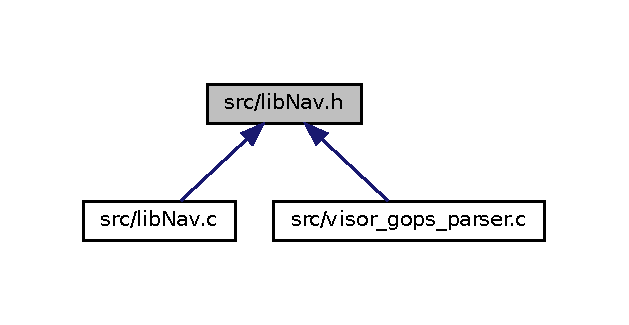
\includegraphics[width=302pt]{libNav_8h__dep__incl}
\end{center}
\end{figure}
\subsection*{Data Structures}
\begin{DoxyCompactItemize}
\item 
struct \hyperlink{structNavigation__Node}{Navigation\-\_\-\-Node}
\begin{DoxyCompactList}\small\item\em Navigation structure with start points, overall size, and current index values. \end{DoxyCompactList}\end{DoxyCompactItemize}
\subsection*{Functions}
\begin{DoxyCompactItemize}
\item 
struct \hyperlink{structNavigation__Node}{Navigation\-\_\-\-Node} $\ast$ \hyperlink{libNav_8h_aa25a9e1e8a1e470352cfdbb88d0f5b5e}{New\-Nav\-Node} ()
\begin{DoxyCompactList}\small\item\em Returns a newly minted \hyperlink{structNode}{Node}. \end{DoxyCompactList}\item 
void \hyperlink{libNav_8h_ad5f3fa84f88ddba51c3163e376b7e278}{Print\-Nav\-Node} (struct \hyperlink{structNavigation__Node}{Navigation\-\_\-\-Node} $\ast$inc\-\_\-nav\-Node\-Ptr)
\begin{DoxyCompactList}\small\item\em Returns meta-\/data about the Navigation \hyperlink{structNode}{Node} to standard output. \end{DoxyCompactList}\end{DoxyCompactItemize}


\subsection{Detailed Description}
Contains definitions for Navigation necessary for tracking position while processing each \char`\"{}slice\char`\"{} of an image. \begin{DoxyAuthor}{Author}
N\-R\-L, Code 7330 
\end{DoxyAuthor}
\begin{DoxyDate}{Date}
2019/05/31 Navigational data regarding overall coordinates of image as well as actual slicing information as the image is parsed.
\end{DoxyDate}
\begin{DoxySeeAlso}{See Also}
\href{https://confluence.di2e.net/display/NRL7331/VISOR}{\tt https\-://confluence.\-di2e.\-net/display/\-N\-R\-L7331/\-V\-I\-S\-O\-R} 
\end{DoxySeeAlso}


Definition in file \hyperlink{libNav_8h_source}{lib\-Nav.\-h}.



\subsection{Function Documentation}
\hypertarget{libNav_8h_aa25a9e1e8a1e470352cfdbb88d0f5b5e}{\index{lib\-Nav.\-h@{lib\-Nav.\-h}!New\-Nav\-Node@{New\-Nav\-Node}}
\index{New\-Nav\-Node@{New\-Nav\-Node}!libNav.h@{lib\-Nav.\-h}}
\subsubsection[{New\-Nav\-Node}]{\setlength{\rightskip}{0pt plus 5cm}struct {\bf Navigation\-\_\-\-Node}$\ast$ New\-Nav\-Node (
\begin{DoxyParamCaption}
{}
\end{DoxyParamCaption}
)}}\label{libNav_8h_aa25a9e1e8a1e470352cfdbb88d0f5b5e}


Returns a newly minted \hyperlink{structNode}{Node}. 

Returns a newly minted \hyperlink{structNode}{Node}.


\begin{DoxyParams}{Parameters}
{\em none} & \\
\hline
\end{DoxyParams}
\begin{DoxyReturn}{Returns}
\hyperlink{structNavigation__Node}{Navigation\-\_\-\-Node} 
\end{DoxyReturn}


Definition at line 73 of file lib\-Nav.\-c.

\hypertarget{libNav_8h_ad5f3fa84f88ddba51c3163e376b7e278}{\index{lib\-Nav.\-h@{lib\-Nav.\-h}!Print\-Nav\-Node@{Print\-Nav\-Node}}
\index{Print\-Nav\-Node@{Print\-Nav\-Node}!libNav.h@{lib\-Nav.\-h}}
\subsubsection[{Print\-Nav\-Node}]{\setlength{\rightskip}{0pt plus 5cm}void Print\-Nav\-Node (
\begin{DoxyParamCaption}
\item[{struct {\bf Navigation\-\_\-\-Node} $\ast$}]{inc\-\_\-nav\-Node\-Ptr}
\end{DoxyParamCaption}
)}}\label{libNav_8h_ad5f3fa84f88ddba51c3163e376b7e278}


Returns meta-\/data about the Navigation \hyperlink{structNode}{Node} to standard output. 

Returns meta-\/data about the Navigation \hyperlink{structNode}{Node} to standard output.


\begin{DoxyParams}{Parameters}
{\em \hyperlink{structNavigation__Node}{Navigation\-\_\-\-Node}} & \\
\hline
\end{DoxyParams}
\begin{DoxyReturn}{Returns}
void 
\end{DoxyReturn}


Definition at line 38 of file lib\-Nav.\-c.


\hypertarget{libProduct_8h}{\section{src/lib\-Product.h File Reference}
\label{libProduct_8h}\index{src/lib\-Product.\-h@{src/lib\-Product.\-h}}
}


Contains definitions for a \hyperlink{structProduct}{Product} structure necessary to hold salient meta-\/data related to a scientific data point. Information is gathered from the Net\-C\-D\-F/\-H\-D\-F5 file for persistence thus ensuring is does have to continually be accessed for the same data.  


This graph shows which files directly or indirectly include this file\-:\nopagebreak
\begin{figure}[H]
\begin{center}
\leavevmode
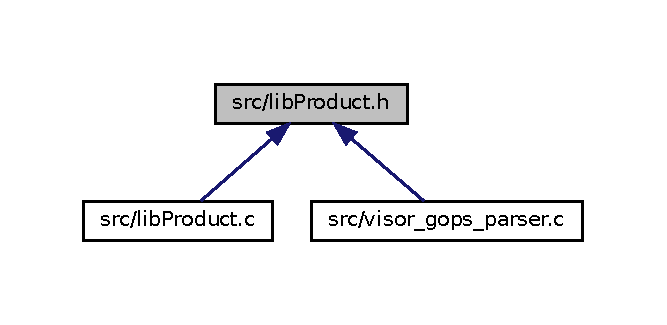
\includegraphics[width=320pt]{libProduct_8h__dep__incl}
\end{center}
\end{figure}
\subsection*{Data Structures}
\begin{DoxyCompactItemize}
\item 
struct \hyperlink{structProduct__Node}{Product\-\_\-\-Node}
\end{DoxyCompactItemize}
\subsection*{Macros}
\begin{DoxyCompactItemize}
\item 
\#define \hyperlink{libProduct_8h_a9db775ed29138af8173b6e9a13d50b43}{A\-T\-T\-\_\-\-N\-M\-\_\-\-S\-C\-A\-L\-E\-\_\-\-F\-A\-C\-T\-O\-R}~\char`\"{}scale\-\_\-factor\char`\"{}
\item 
\#define \hyperlink{libProduct_8h_aa2a42c8375e7ce6df89b3e078c8baebf}{A\-T\-T\-\_\-\-N\-M\-\_\-\-A\-D\-D\-\_\-\-O\-F\-F\-S\-E\-T}~\char`\"{}add\-\_\-offset\char`\"{}
\item 
\#define \hyperlink{libProduct_8h_a8c41f7047ace1bd9d8a468706351e7d1}{A\-T\-T\-\_\-\-N\-M\-\_\-\-M\-A\-X\-\_\-\-S\-I\-Z\-E}~255
\item 
\#define \hyperlink{libProduct_8h_a5b63207c5ee57a1a43ae61b697f046c9}{P\-R\-O\-D\-U\-C\-T\-\_\-\-F\-I\-L\-L\-\_\-\-V\-A\-L\-U\-E}~-\/32767
\end{DoxyCompactItemize}
\subsection*{Typedefs}
\begin{DoxyCompactItemize}
\item 
\hypertarget{libProduct_8h_a78a43077ff2f12332d23106cb4aab9c3}{typedef struct \hyperlink{structProduct__Node}{Product\-\_\-\-Node} $\ast$ {\bfseries prod\-Ptr}}\label{libProduct_8h_a78a43077ff2f12332d23106cb4aab9c3}

\end{DoxyCompactItemize}
\subsection*{Functions}
\begin{DoxyCompactItemize}
\item 
\hypertarget{libProduct_8h_aa5a994d345c27e96aed658adf4a4b67d}{\hyperlink{structProduct__Node}{prod\-Ptr} \hyperlink{libProduct_8h_aa5a994d345c27e96aed658adf4a4b67d}{New\-Product\-Node} ()}\label{libProduct_8h_aa5a994d345c27e96aed658adf4a4b67d}

\begin{DoxyCompactList}\small\item\em Creates a new \hyperlink{structProduct}{Product} \hyperlink{structNode}{Node} for storage of meta-\/data related to a product passed. \end{DoxyCompactList}\item 
void \hyperlink{libProduct_8h_a59424c2f92072709165acca6c0f78c34}{Print\-Product\-Node} (const \hyperlink{structProduct__Node}{prod\-Ptr} inc\-\_\-prod\-Ptr)
\begin{DoxyCompactList}\small\item\em Prints each node to standard output for lat, long, and optics value. \end{DoxyCompactList}\item 
void \hyperlink{libProduct_8h_adb284521fd68ca8e0bac06cbbd0fe5c9}{Free\-Product\-Node} (const \hyperlink{structProduct__Node}{prod\-Ptr} inc\-\_\-prod\-Ptr)
\begin{DoxyCompactList}\small\item\em Iterates through each -\/$>$next reference and frees memory. \end{DoxyCompactList}\end{DoxyCompactItemize}


\subsection{Detailed Description}
Contains definitions for a \hyperlink{structProduct}{Product} structure necessary to hold salient meta-\/data related to a scientific data point. Information is gathered from the Net\-C\-D\-F/\-H\-D\-F5 file for persistence thus ensuring is does have to continually be accessed for the same data. \begin{DoxyAuthor}{Author}
N\-R\-L, Code 7330 
\end{DoxyAuthor}
\begin{DoxyDate}{Date}
2019/05/31 Library used to store information about a product gathered from the parent Net\-C\-D\-F/\-H\-D\-F5 file and persisted to support optics data processing as the satellite file is parsed into individual slices.
\end{DoxyDate}
\begin{DoxySeeAlso}{See Also}
\href{https://confluence.di2e.net/display/NRL7331/VISOR}{\tt https\-://confluence.\-di2e.\-net/display/\-N\-R\-L7331/\-V\-I\-S\-O\-R} 
\end{DoxySeeAlso}


Definition in file \hyperlink{libProduct_8h_source}{lib\-Product.\-h}.



\subsection{Macro Definition Documentation}
\hypertarget{libProduct_8h_aa2a42c8375e7ce6df89b3e078c8baebf}{\index{lib\-Product.\-h@{lib\-Product.\-h}!A\-T\-T\-\_\-\-N\-M\-\_\-\-A\-D\-D\-\_\-\-O\-F\-F\-S\-E\-T@{A\-T\-T\-\_\-\-N\-M\-\_\-\-A\-D\-D\-\_\-\-O\-F\-F\-S\-E\-T}}
\index{A\-T\-T\-\_\-\-N\-M\-\_\-\-A\-D\-D\-\_\-\-O\-F\-F\-S\-E\-T@{A\-T\-T\-\_\-\-N\-M\-\_\-\-A\-D\-D\-\_\-\-O\-F\-F\-S\-E\-T}!libProduct.h@{lib\-Product.\-h}}
\subsubsection[{A\-T\-T\-\_\-\-N\-M\-\_\-\-A\-D\-D\-\_\-\-O\-F\-F\-S\-E\-T}]{\setlength{\rightskip}{0pt plus 5cm}\#define A\-T\-T\-\_\-\-N\-M\-\_\-\-A\-D\-D\-\_\-\-O\-F\-F\-S\-E\-T~\char`\"{}add\-\_\-offset\char`\"{}}}\label{libProduct_8h_aa2a42c8375e7ce6df89b3e078c8baebf}
Actual name of variable from within input file. 

Definition at line 37 of file lib\-Product.\-h.

\hypertarget{libProduct_8h_a8c41f7047ace1bd9d8a468706351e7d1}{\index{lib\-Product.\-h@{lib\-Product.\-h}!A\-T\-T\-\_\-\-N\-M\-\_\-\-M\-A\-X\-\_\-\-S\-I\-Z\-E@{A\-T\-T\-\_\-\-N\-M\-\_\-\-M\-A\-X\-\_\-\-S\-I\-Z\-E}}
\index{A\-T\-T\-\_\-\-N\-M\-\_\-\-M\-A\-X\-\_\-\-S\-I\-Z\-E@{A\-T\-T\-\_\-\-N\-M\-\_\-\-M\-A\-X\-\_\-\-S\-I\-Z\-E}!libProduct.h@{lib\-Product.\-h}}
\subsubsection[{A\-T\-T\-\_\-\-N\-M\-\_\-\-M\-A\-X\-\_\-\-S\-I\-Z\-E}]{\setlength{\rightskip}{0pt plus 5cm}\#define A\-T\-T\-\_\-\-N\-M\-\_\-\-M\-A\-X\-\_\-\-S\-I\-Z\-E~255}}\label{libProduct_8h_a8c41f7047ace1bd9d8a468706351e7d1}
Defined maximum size of any attribute for purposes of defining string space. 

Definition at line 38 of file lib\-Product.\-h.

\hypertarget{libProduct_8h_a9db775ed29138af8173b6e9a13d50b43}{\index{lib\-Product.\-h@{lib\-Product.\-h}!A\-T\-T\-\_\-\-N\-M\-\_\-\-S\-C\-A\-L\-E\-\_\-\-F\-A\-C\-T\-O\-R@{A\-T\-T\-\_\-\-N\-M\-\_\-\-S\-C\-A\-L\-E\-\_\-\-F\-A\-C\-T\-O\-R}}
\index{A\-T\-T\-\_\-\-N\-M\-\_\-\-S\-C\-A\-L\-E\-\_\-\-F\-A\-C\-T\-O\-R@{A\-T\-T\-\_\-\-N\-M\-\_\-\-S\-C\-A\-L\-E\-\_\-\-F\-A\-C\-T\-O\-R}!libProduct.h@{lib\-Product.\-h}}
\subsubsection[{A\-T\-T\-\_\-\-N\-M\-\_\-\-S\-C\-A\-L\-E\-\_\-\-F\-A\-C\-T\-O\-R}]{\setlength{\rightskip}{0pt plus 5cm}\#define A\-T\-T\-\_\-\-N\-M\-\_\-\-S\-C\-A\-L\-E\-\_\-\-F\-A\-C\-T\-O\-R~\char`\"{}scale\-\_\-factor\char`\"{}}}\label{libProduct_8h_a9db775ed29138af8173b6e9a13d50b43}
Actual name of variable from within input file. 

Definition at line 36 of file lib\-Product.\-h.

\hypertarget{libProduct_8h_a5b63207c5ee57a1a43ae61b697f046c9}{\index{lib\-Product.\-h@{lib\-Product.\-h}!P\-R\-O\-D\-U\-C\-T\-\_\-\-F\-I\-L\-L\-\_\-\-V\-A\-L\-U\-E@{P\-R\-O\-D\-U\-C\-T\-\_\-\-F\-I\-L\-L\-\_\-\-V\-A\-L\-U\-E}}
\index{P\-R\-O\-D\-U\-C\-T\-\_\-\-F\-I\-L\-L\-\_\-\-V\-A\-L\-U\-E@{P\-R\-O\-D\-U\-C\-T\-\_\-\-F\-I\-L\-L\-\_\-\-V\-A\-L\-U\-E}!libProduct.h@{lib\-Product.\-h}}
\subsubsection[{P\-R\-O\-D\-U\-C\-T\-\_\-\-F\-I\-L\-L\-\_\-\-V\-A\-L\-U\-E}]{\setlength{\rightskip}{0pt plus 5cm}\#define P\-R\-O\-D\-U\-C\-T\-\_\-\-F\-I\-L\-L\-\_\-\-V\-A\-L\-U\-E~-\/32767}}\label{libProduct_8h_a5b63207c5ee57a1a43ae61b697f046c9}
Defined universal integer value for \char`\"{}fills\char`\"{} in data. 

Definition at line 39 of file lib\-Product.\-h.



\subsection{Function Documentation}
\hypertarget{libProduct_8h_adb284521fd68ca8e0bac06cbbd0fe5c9}{\index{lib\-Product.\-h@{lib\-Product.\-h}!Free\-Product\-Node@{Free\-Product\-Node}}
\index{Free\-Product\-Node@{Free\-Product\-Node}!libProduct.h@{lib\-Product.\-h}}
\subsubsection[{Free\-Product\-Node}]{\setlength{\rightskip}{0pt plus 5cm}void Free\-Product\-Node (
\begin{DoxyParamCaption}
\item[{const {\bf prod\-Ptr}}]{inc\-\_\-prod\-Ptr}
\end{DoxyParamCaption}
)}}\label{libProduct_8h_adb284521fd68ca8e0bac06cbbd0fe5c9}


Iterates through each -\/$>$next reference and frees memory. 

Iterates through each -\/$>$next reference and frees memory.


\begin{DoxyParams}{Parameters}
{\em const} & prod\-Ptr -\/ incoming product pointer \\
\hline
\end{DoxyParams}
\begin{DoxyReturn}{Returns}
void 
\end{DoxyReturn}


Definition at line 40 of file lib\-Product.\-c.

\hypertarget{libProduct_8h_a59424c2f92072709165acca6c0f78c34}{\index{lib\-Product.\-h@{lib\-Product.\-h}!Print\-Product\-Node@{Print\-Product\-Node}}
\index{Print\-Product\-Node@{Print\-Product\-Node}!libProduct.h@{lib\-Product.\-h}}
\subsubsection[{Print\-Product\-Node}]{\setlength{\rightskip}{0pt plus 5cm}void Print\-Product\-Node (
\begin{DoxyParamCaption}
\item[{const {\bf prod\-Ptr}}]{inc\-\_\-prod\-Ptr}
\end{DoxyParamCaption}
)}}\label{libProduct_8h_a59424c2f92072709165acca6c0f78c34}


Prints each node to standard output for lat, long, and optics value. 

Prints each node to standard output for lat, long, and optics value.


\begin{DoxyParams}{Parameters}
{\em const} & prod\-Ptr -\/ incoming product pointer to print \\
\hline
\end{DoxyParams}
\begin{DoxyReturn}{Returns}
void 
\end{DoxyReturn}


Definition at line 51 of file lib\-Product.\-c.


\hypertarget{log_8h}{\section{src/log.h File Reference}
\label{log_8h}\index{src/log.\-h@{src/log.\-h}}
}


Contains definitions for Nodes used in a Linked List.  


{\ttfamily \#include $<$stdio.\-h$>$}\\*
{\ttfamily \#include $<$stdarg.\-h$>$}\\*
Include dependency graph for log.\-h\-:\nopagebreak
\begin{figure}[H]
\begin{center}
\leavevmode
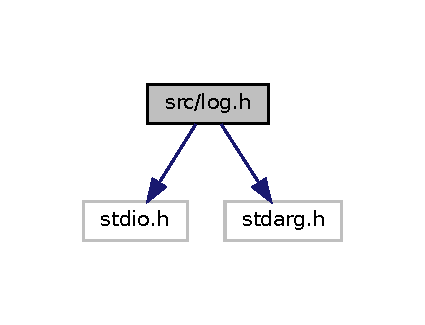
\includegraphics[width=204pt]{log_8h__incl}
\end{center}
\end{figure}
This graph shows which files directly or indirectly include this file\-:\nopagebreak
\begin{figure}[H]
\begin{center}
\leavevmode
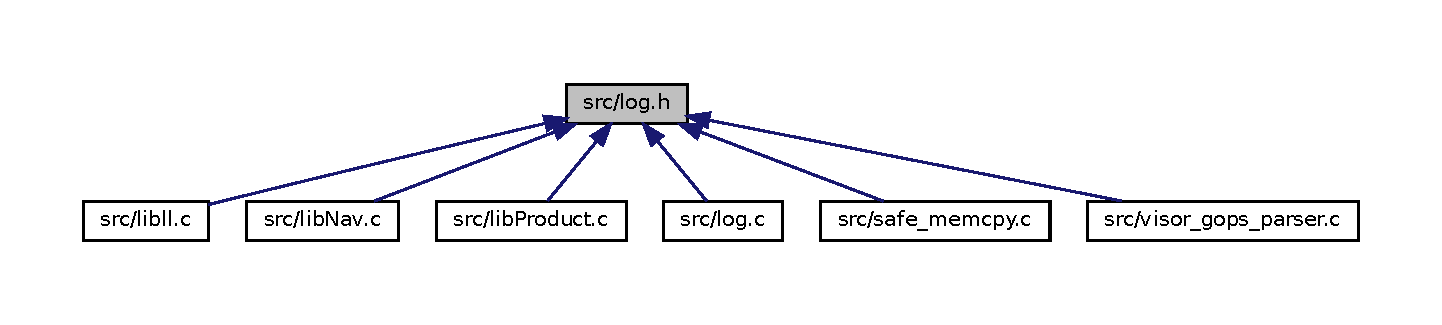
\includegraphics[width=350pt]{log_8h__dep__incl}
\end{center}
\end{figure}
\subsection*{Macros}
\begin{DoxyCompactItemize}
\item 
\hypertarget{log_8h_aa48b2017856a8a9c33a9935afe604c8d}{\#define {\bfseries L\-O\-G\-\_\-\-V\-E\-R\-S\-I\-O\-N}~\char`\"{}0.\-1.\-0\char`\"{}}\label{log_8h_aa48b2017856a8a9c33a9935afe604c8d}

\item 
\hypertarget{log_8h_af89cb876e6e1d43cfeacdd58a7c9b78c}{\#define {\bfseries log\-\_\-trace}(...)~log\-\_\-log(L\-O\-G\-\_\-\-T\-R\-A\-C\-E, \-\_\-\-\_\-\-F\-I\-L\-E\-\_\-\-\_\-, \-\_\-\-\_\-\-L\-I\-N\-E\-\_\-\-\_\-, \-\_\-\-\_\-\-V\-A\-\_\-\-A\-R\-G\-S\-\_\-\-\_\-)}\label{log_8h_af89cb876e6e1d43cfeacdd58a7c9b78c}

\item 
\hypertarget{log_8h_aa77e596ef13d2f0f75d0ac9540ed358d}{\#define {\bfseries log\-\_\-debug}(...)~log\-\_\-log(L\-O\-G\-\_\-\-D\-E\-B\-U\-G, \-\_\-\-\_\-\-F\-I\-L\-E\-\_\-\-\_\-, \-\_\-\-\_\-\-L\-I\-N\-E\-\_\-\-\_\-, \-\_\-\-\_\-\-V\-A\-\_\-\-A\-R\-G\-S\-\_\-\-\_\-)}\label{log_8h_aa77e596ef13d2f0f75d0ac9540ed358d}

\item 
\hypertarget{log_8h_aa1cfe5444875c8eca0ea6f6993977d6d}{\#define {\bfseries log\-\_\-info}(...)~log\-\_\-log(L\-O\-G\-\_\-\-I\-N\-F\-O, \-\_\-\-\_\-\-F\-I\-L\-E\-\_\-\-\_\-, \-\_\-\-\_\-\-L\-I\-N\-E\-\_\-\-\_\-, \-\_\-\-\_\-\-V\-A\-\_\-\-A\-R\-G\-S\-\_\-\-\_\-)}\label{log_8h_aa1cfe5444875c8eca0ea6f6993977d6d}

\item 
\hypertarget{log_8h_a04af09851c431d178f16b24fa1aac1e9}{\#define {\bfseries log\-\_\-warn}(...)~log\-\_\-log(L\-O\-G\-\_\-\-W\-A\-R\-N, \-\_\-\-\_\-\-F\-I\-L\-E\-\_\-\-\_\-, \-\_\-\-\_\-\-L\-I\-N\-E\-\_\-\-\_\-, \-\_\-\-\_\-\-V\-A\-\_\-\-A\-R\-G\-S\-\_\-\-\_\-)}\label{log_8h_a04af09851c431d178f16b24fa1aac1e9}

\item 
\hypertarget{log_8h_a6ae72553ea9805dd87a463d6f710364d}{\#define {\bfseries log\-\_\-error}(...)~log\-\_\-log(L\-O\-G\-\_\-\-E\-R\-R\-O\-R, \-\_\-\-\_\-\-F\-I\-L\-E\-\_\-\-\_\-, \-\_\-\-\_\-\-L\-I\-N\-E\-\_\-\-\_\-, \-\_\-\-\_\-\-V\-A\-\_\-\-A\-R\-G\-S\-\_\-\-\_\-)}\label{log_8h_a6ae72553ea9805dd87a463d6f710364d}

\item 
\hypertarget{log_8h_a704a43b1e2ff3bb554aff101efdbeecf}{\#define {\bfseries log\-\_\-fatal}(...)~log\-\_\-log(L\-O\-G\-\_\-\-F\-A\-T\-A\-L, \-\_\-\-\_\-\-F\-I\-L\-E\-\_\-\-\_\-, \-\_\-\-\_\-\-L\-I\-N\-E\-\_\-\-\_\-, \-\_\-\-\_\-\-V\-A\-\_\-\-A\-R\-G\-S\-\_\-\-\_\-)}\label{log_8h_a704a43b1e2ff3bb554aff101efdbeecf}

\item 
\hypertarget{log_8h_af2ca793fa591cec3c25b023fd03787c9}{\#define {\bfseries log\-\_\-emerg}(...)~log\-\_\-log(L\-O\-G\-\_\-\-F\-A\-T\-A\-L, \-\_\-\-\_\-\-F\-I\-L\-E\-\_\-\-\_\-, \-\_\-\-\_\-\-L\-I\-N\-E\-\_\-\-\_\-, \-\_\-\-\_\-\-V\-A\-\_\-\-A\-R\-G\-S\-\_\-\-\_\-)}\label{log_8h_af2ca793fa591cec3c25b023fd03787c9}

\end{DoxyCompactItemize}
\subsection*{Typedefs}
\begin{DoxyCompactItemize}
\item 
\hypertarget{log_8h_ae4814768d44b3dc4fc107e713de0477f}{typedef void($\ast$ {\bfseries log\-\_\-\-Lock\-Fn} )(void $\ast$udata, int lock)}\label{log_8h_ae4814768d44b3dc4fc107e713de0477f}

\end{DoxyCompactItemize}
\subsection*{Enumerations}
\begin{DoxyCompactItemize}
\item 
enum \{ \\*
{\bfseries L\-O\-G\-\_\-\-T\-R\-A\-C\-E}, 
{\bfseries L\-O\-G\-\_\-\-D\-E\-B\-U\-G}, 
{\bfseries L\-O\-G\-\_\-\-I\-N\-F\-O}, 
{\bfseries L\-O\-G\-\_\-\-W\-A\-R\-N}, 
\\*
{\bfseries L\-O\-G\-\_\-\-E\-R\-R\-O\-R}, 
{\bfseries L\-O\-G\-\_\-\-F\-A\-T\-A\-L}
 \}
\end{DoxyCompactItemize}
\subsection*{Functions}
\begin{DoxyCompactItemize}
\item 
\hypertarget{log_8h_a670c547ace6683148e5f480c4fc4c0f0}{void {\bfseries log\-\_\-set\-\_\-udata} (void $\ast$udata)}\label{log_8h_a670c547ace6683148e5f480c4fc4c0f0}

\item 
\hypertarget{log_8h_a93d6674a530b372c85e6bdf275e6e6b4}{void {\bfseries log\-\_\-set\-\_\-lock} (log\-\_\-\-Lock\-Fn fn)}\label{log_8h_a93d6674a530b372c85e6bdf275e6e6b4}

\item 
\hypertarget{log_8h_af0f33363d4098787cac5b47f0a6ad443}{void {\bfseries log\-\_\-set\-\_\-fp} (F\-I\-L\-E $\ast$fp)}\label{log_8h_af0f33363d4098787cac5b47f0a6ad443}

\item 
\hypertarget{log_8h_af2493e94f152a28b2ba4e3a2e2bba65d}{void {\bfseries log\-\_\-set\-\_\-level} (int level)}\label{log_8h_af2493e94f152a28b2ba4e3a2e2bba65d}

\item 
\hypertarget{log_8h_a15fc2e61d925edc83d6eaa748a7fb40c}{void {\bfseries log\-\_\-set\-\_\-quiet} (int enable)}\label{log_8h_a15fc2e61d925edc83d6eaa748a7fb40c}

\item 
\hypertarget{log_8h_ac008ecbde449b2dd1bc4f8671d9a0e07}{void {\bfseries log\-\_\-log} (int level, const char $\ast$file, int line, const char $\ast$fmt,...)}\label{log_8h_ac008ecbde449b2dd1bc4f8671d9a0e07}

\end{DoxyCompactItemize}


\subsection{Detailed Description}
Contains definitions for Nodes used in a Linked List. \begin{DoxyAuthor}{Author}
N\-R\-L, Code 7330 
\end{DoxyAuthor}
\begin{DoxyDate}{Date}
2019/05/31 Copyright (c) 2017 rxi
\end{DoxyDate}
This library is free software; you can redistribute it and/or modify it under the terms of the M\-I\-T license. See {\ttfamily \hyperlink{log_8c_source}{log.\-c}} for details.

Logging library used from, see reference blow, another project to support granular logging.

\begin{DoxySeeAlso}{See Also}
\href{https://github.com/rxi/log.c}{\tt https\-://github.\-com/rxi/log.\-c} 
\end{DoxySeeAlso}


Definition in file \hyperlink{log_8h_source}{log.\-h}.


\hypertarget{safe__memcpy_8h}{\section{src/safe\-\_\-memcpy.h File Reference}
\label{safe__memcpy_8h}\index{src/safe\-\_\-memcpy.\-h@{src/safe\-\_\-memcpy.\-h}}
}


Contains definitions for safe memory copy of strings.  


This graph shows which files directly or indirectly include this file\-:\nopagebreak
\begin{figure}[H]
\begin{center}
\leavevmode
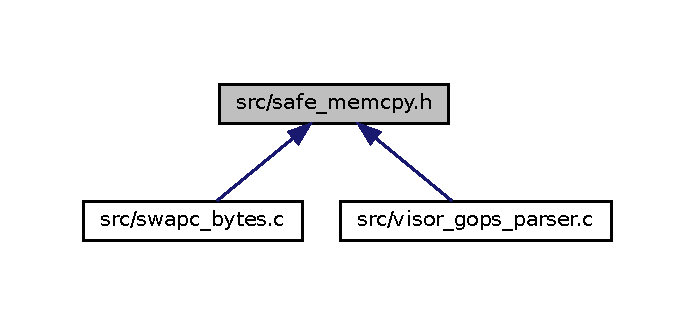
\includegraphics[width=334pt]{safe__memcpy_8h__dep__incl}
\end{center}
\end{figure}
\subsection*{Functions}
\begin{DoxyCompactItemize}
\item 
int \hyperlink{safe__memcpy_8h_ab1681eaee16d7efe6bd5659c1ce28174}{safe\-\_\-memcpy} (char $\ast$dest, const char $\ast$src, size\-\_\-t cnt)
\begin{DoxyCompactList}\small\item\em Local implementation of a safe memory copy procedure, wrapper. \end{DoxyCompactList}\end{DoxyCompactItemize}


\subsection{Detailed Description}
Contains definitions for safe memory copy of strings. \begin{DoxyAuthor}{Author}
N\-R\-L, Code 7330 
\end{DoxyAuthor}
\begin{DoxyDate}{Date}
2021/04/19 Security wrapper for protected memory copy functions.
\end{DoxyDate}
\begin{DoxySeeAlso}{See Also}
\href{https://confluence.di2e.net/display/NRL7331/VISOR}{\tt https\-://confluence.\-di2e.\-net/display/\-N\-R\-L7331/\-V\-I\-S\-O\-R} 
\end{DoxySeeAlso}


Definition in file \hyperlink{safe__memcpy_8h_source}{safe\-\_\-memcpy.\-h}.



\subsection{Function Documentation}
\hypertarget{safe__memcpy_8h_ab1681eaee16d7efe6bd5659c1ce28174}{\index{safe\-\_\-memcpy.\-h@{safe\-\_\-memcpy.\-h}!safe\-\_\-memcpy@{safe\-\_\-memcpy}}
\index{safe\-\_\-memcpy@{safe\-\_\-memcpy}!safe_memcpy.h@{safe\-\_\-memcpy.\-h}}
\subsubsection[{safe\-\_\-memcpy}]{\setlength{\rightskip}{0pt plus 5cm}int safe\-\_\-memcpy (
\begin{DoxyParamCaption}
\item[{char $\ast$}]{dest, }
\item[{const char $\ast$}]{src, }
\item[{size\-\_\-t}]{cnt}
\end{DoxyParamCaption}
)}}\label{safe__memcpy_8h_ab1681eaee16d7efe6bd5659c1ce28174}


Local implementation of a safe memory copy procedure, wrapper. 

Local implementation of a safe memory copy procedure, wrapper.


\begin{DoxyParams}{Parameters}
{\em char} & $\ast$ dest -\/ target data \\
\hline
{\em const} & char $\ast$ src -\/ source data \\
\hline
{\em size\-\_\-t} & cnt -\/ number of bytes to copy \\
\hline
\end{DoxyParams}
\begin{DoxyReturn}{Returns}
void 
\end{DoxyReturn}


Definition at line 45 of file safe\-\_\-memcpy.\-c.



Here is the caller graph for this function\-:\nopagebreak
\begin{figure}[H]
\begin{center}
\leavevmode
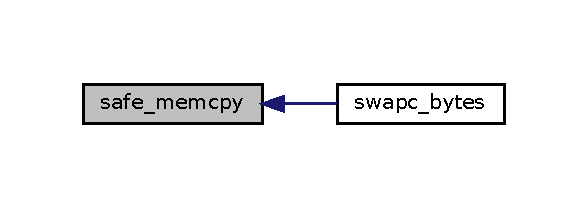
\includegraphics[width=282pt]{safe__memcpy_8h_ab1681eaee16d7efe6bd5659c1ce28174_icgraph}
\end{center}
\end{figure}



\hypertarget{swapc__bytes_8h}{\section{src/swapc\-\_\-bytes.h File Reference}
\label{swapc__bytes_8h}\index{src/swapc\-\_\-bytes.\-h@{src/swapc\-\_\-bytes.\-h}}
}


Routines for swapping bytes due to endianess requirements of project.  


This graph shows which files directly or indirectly include this file\-:\nopagebreak
\begin{figure}[H]
\begin{center}
\leavevmode
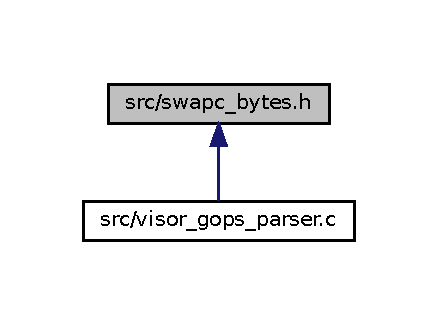
\includegraphics[width=210pt]{swapc__bytes_8h__dep__incl}
\end{center}
\end{figure}
\subsection*{Functions}
\begin{DoxyCompactItemize}
\item 
void \hyperlink{swapc__bytes_8h_a06c33eac02176dea763880121a447805}{swapc\-\_\-bytes} (char $\ast$in, int nbyte, int ntime)
\begin{DoxyCompactList}\small\item\em Swaps bytes given a pointer, number of bytes and size of swaps to make. \end{DoxyCompactList}\item 
void \hyperlink{swapc__bytes_8h_a05408c9b7872f382b58aa7af5e514a49}{swapc\-\_\-bytes2} (const char $\ast$in, char $\ast$out, int nbyte, int ntime)
\begin{DoxyCompactList}\small\item\em Swaps bytes given a pointer but doesn't change anything in the original value given (allocate memory!) \end{DoxyCompactList}\item 
int \hyperlink{swapc__bytes_8h_ab1681eaee16d7efe6bd5659c1ce28174}{safe\-\_\-memcpy} (char $\ast$dest, const char $\ast$src, size\-\_\-t cnt)
\begin{DoxyCompactList}\small\item\em Wrapper for memory copies done safely with layered defense, return on non-\/zero is an error. \end{DoxyCompactList}\end{DoxyCompactItemize}


\subsection{Detailed Description}
Routines for swapping bytes due to endianess requirements of project. \begin{DoxyAuthor}{Author}
N\-R\-L, Code 7330 
\end{DoxyAuthor}
\begin{DoxyDate}{Date}
2019/05/31 Routines pulled from satellite image processing code\-: 
\end{DoxyDate}
\begin{DoxySeeAlso}{See Also}
/export/projects/socom/aps7/ocssw/oel\-\_\-util/libgenutils/swapc\-\_\-bytes.c

\href{https://confluence.di2e.net/display/NRL7331/VISOR}{\tt https\-://confluence.\-di2e.\-net/display/\-N\-R\-L7331/\-V\-I\-S\-O\-R} 
\end{DoxySeeAlso}


Definition in file \hyperlink{swapc__bytes_8h_source}{swapc\-\_\-bytes.\-h}.



\subsection{Function Documentation}
\hypertarget{swapc__bytes_8h_ab1681eaee16d7efe6bd5659c1ce28174}{\index{swapc\-\_\-bytes.\-h@{swapc\-\_\-bytes.\-h}!safe\-\_\-memcpy@{safe\-\_\-memcpy}}
\index{safe\-\_\-memcpy@{safe\-\_\-memcpy}!swapc_bytes.h@{swapc\-\_\-bytes.\-h}}
\subsubsection[{safe\-\_\-memcpy}]{\setlength{\rightskip}{0pt plus 5cm}int safe\-\_\-memcpy (
\begin{DoxyParamCaption}
\item[{char $\ast$}]{dest, }
\item[{const char $\ast$}]{src, }
\item[{size\-\_\-t}]{cnt}
\end{DoxyParamCaption}
)}}\label{swapc__bytes_8h_ab1681eaee16d7efe6bd5659c1ce28174}


Wrapper for memory copies done safely with layered defense, return on non-\/zero is an error. 

Local implementation of a safe memory copy procedure, wrapper.


\begin{DoxyParams}{Parameters}
{\em char} & $\ast$ dest -\/ target data \\
\hline
{\em const} & char $\ast$ src -\/ source data \\
\hline
{\em size\-\_\-t} & cnt -\/ number of bytes to copy \\
\hline
\end{DoxyParams}
\begin{DoxyReturn}{Returns}
void 
\end{DoxyReturn}


Definition at line 45 of file safe\-\_\-memcpy.\-c.

\hypertarget{swapc__bytes_8h_a06c33eac02176dea763880121a447805}{\index{swapc\-\_\-bytes.\-h@{swapc\-\_\-bytes.\-h}!swapc\-\_\-bytes@{swapc\-\_\-bytes}}
\index{swapc\-\_\-bytes@{swapc\-\_\-bytes}!swapc_bytes.h@{swapc\-\_\-bytes.\-h}}
\subsubsection[{swapc\-\_\-bytes}]{\setlength{\rightskip}{0pt plus 5cm}void swapc\-\_\-bytes (
\begin{DoxyParamCaption}
\item[{char $\ast$}]{in, }
\item[{int}]{nbyte, }
\item[{int}]{ntime}
\end{DoxyParamCaption}
)}}\label{swapc__bytes_8h_a06c33eac02176dea763880121a447805}


Swaps bytes given a pointer, number of bytes and size of swaps to make. 


\begin{DoxyParams}{Parameters}
{\em char$\ast$} & -\/ pointer to the data itself \\
\hline
{\em int} & -\/ number of bytes that will be swapped (defines incoming data size) \\
\hline
{\em int} & -\/ number of times to swap \\
\hline
\end{DoxyParams}


Definition at line 41 of file swapc\-\_\-bytes.\-c.



Here is the call graph for this function\-:\nopagebreak
\begin{figure}[H]
\begin{center}
\leavevmode
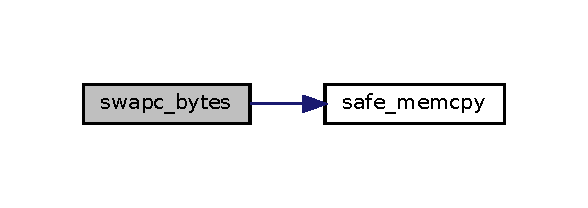
\includegraphics[width=282pt]{swapc__bytes_8h_a06c33eac02176dea763880121a447805_cgraph}
\end{center}
\end{figure}


\hypertarget{swapc__bytes_8h_a05408c9b7872f382b58aa7af5e514a49}{\index{swapc\-\_\-bytes.\-h@{swapc\-\_\-bytes.\-h}!swapc\-\_\-bytes2@{swapc\-\_\-bytes2}}
\index{swapc\-\_\-bytes2@{swapc\-\_\-bytes2}!swapc_bytes.h@{swapc\-\_\-bytes.\-h}}
\subsubsection[{swapc\-\_\-bytes2}]{\setlength{\rightskip}{0pt plus 5cm}void swapc\-\_\-bytes2 (
\begin{DoxyParamCaption}
\item[{const char $\ast$}]{in, }
\item[{char $\ast$}]{out, }
\item[{int}]{nbyte, }
\item[{int}]{ntime}
\end{DoxyParamCaption}
)}}\label{swapc__bytes_8h_a05408c9b7872f382b58aa7af5e514a49}


Swaps bytes given a pointer but doesn't change anything in the original value given (allocate memory!) 


\begin{DoxyParams}{Parameters}
{\em char$\ast$} & -\/ pointer to the data itself \\
\hline
{\em char$\ast$} & -\/ pointer to the new data you want swapped \\
\hline
{\em int} & -\/ number of bytes that will be swapped (defines incoming data size) \\
\hline
{\em int} & -\/ number of times to swap \\
\hline
\end{DoxyParams}


Definition at line 66 of file swapc\-\_\-bytes.\-c.


%--- End generated contents ---

% Index
\newpage
\phantomsection
\addcontentsline{toc}{part}{Index}
\printindex

\end{document}
